% !TEX TS-program = lualatex
% !TEX encoding = UTF-8

\documentclass[psalterium-festivum.tex]{subfiles}

\ifcsname preamble@file\endcsname
  \setcounter{page}{\getpagerefnumber{M-pd36_officium_defunctorum}}
\fi

\begin{document}
\feast{ODEF}{Officium Defunctorum}
	{Officium Defunctorum}{Officium Defunctorum}{2}{}
	{}{}{Defunctorum!Officium}
	{}{}
\addcontentsline{toc}{section}{Officium Defunctorum}

\rubric{Nocturni inferius positi omnes dici possunt, vel etiam unus tantum.}

\gscore{ODEFI}{I}{}{Regem cui omnia vivunt}
\rubric{Non dicitur Hymnus in Officio Defunctorum.}
\vspace{0.5\baselineskip}
\nocturn{1}
\smalltitle{Pro Dominica, Feria \Rnum{2} et \Rnum{5}}
\vspace{0.5\baselineskip}
\gscore{ODEFN1A1}{A}{1}{Dirige Domine}
\psalmus{5}{def}
\gscore{ODEFN1A2}{A}{2}{Convertere Domine}
\psalmus{6}{def}
\vspace{\baselineskip}
\gscore{ODEFN1A3}{A}{3}{Nequando rapiat}
\psalmus{7}{def}
\versiculus{A \textit{porta} \textbf{ín}feri.}{Erue, Dómine, áni\textit{mas e}\textbf{ó}rum.}

\nocturn{2}
\smalltitle{Pro Feria \Rnum{3} et \Rnum{6}}
\gscore{ODEFN2A1}{A}{4}{In loco pascuae}
\psalmus{22}{def}
\vspace{2\baselineskip}
\gscore{ODEFN2A2}{A}{5}{Delicta juventutis meae}
\vspace{\baselineskip}
\psalmus{24}{def}
\vspace{4\baselineskip}
\gscore{Q6F7N2A2}{A}{6}{Credo videre}
\pagebreak\null\par
\psalmus{26}{def}
\versiculus{Cóllocet eos Dóminus \textit{cum prin}\textbf{cí}pibus.}{Cum princípibus pó\textit{puli} \textbf{su}i.}
\pagebreak

\null\par
\nocturn{3}
\smalltitle{Pro Feria \Rnum{4} et Sabbato}
\gscore{ODEFN3A1}{A}{7}{Complaceat tibi}
\psalmus{39}{def}
\gscore{ODEFN3A2}{A}{8}{Sana Domine animam}
\psalmus{40}{def}
\gscore{ODEFN3A3}{A}{9}{Sitivit anima mea}
\psalmus{41}{def}

\vfill
\versiculus{Ne tradas béstiis ánimas confi\textit{téntes} \textbf{ti}bi.}{Et ánimas páuperum tuórum ne obliviscá\textit{ris in} \textbf{fi}nem.}
\vfill

{\centering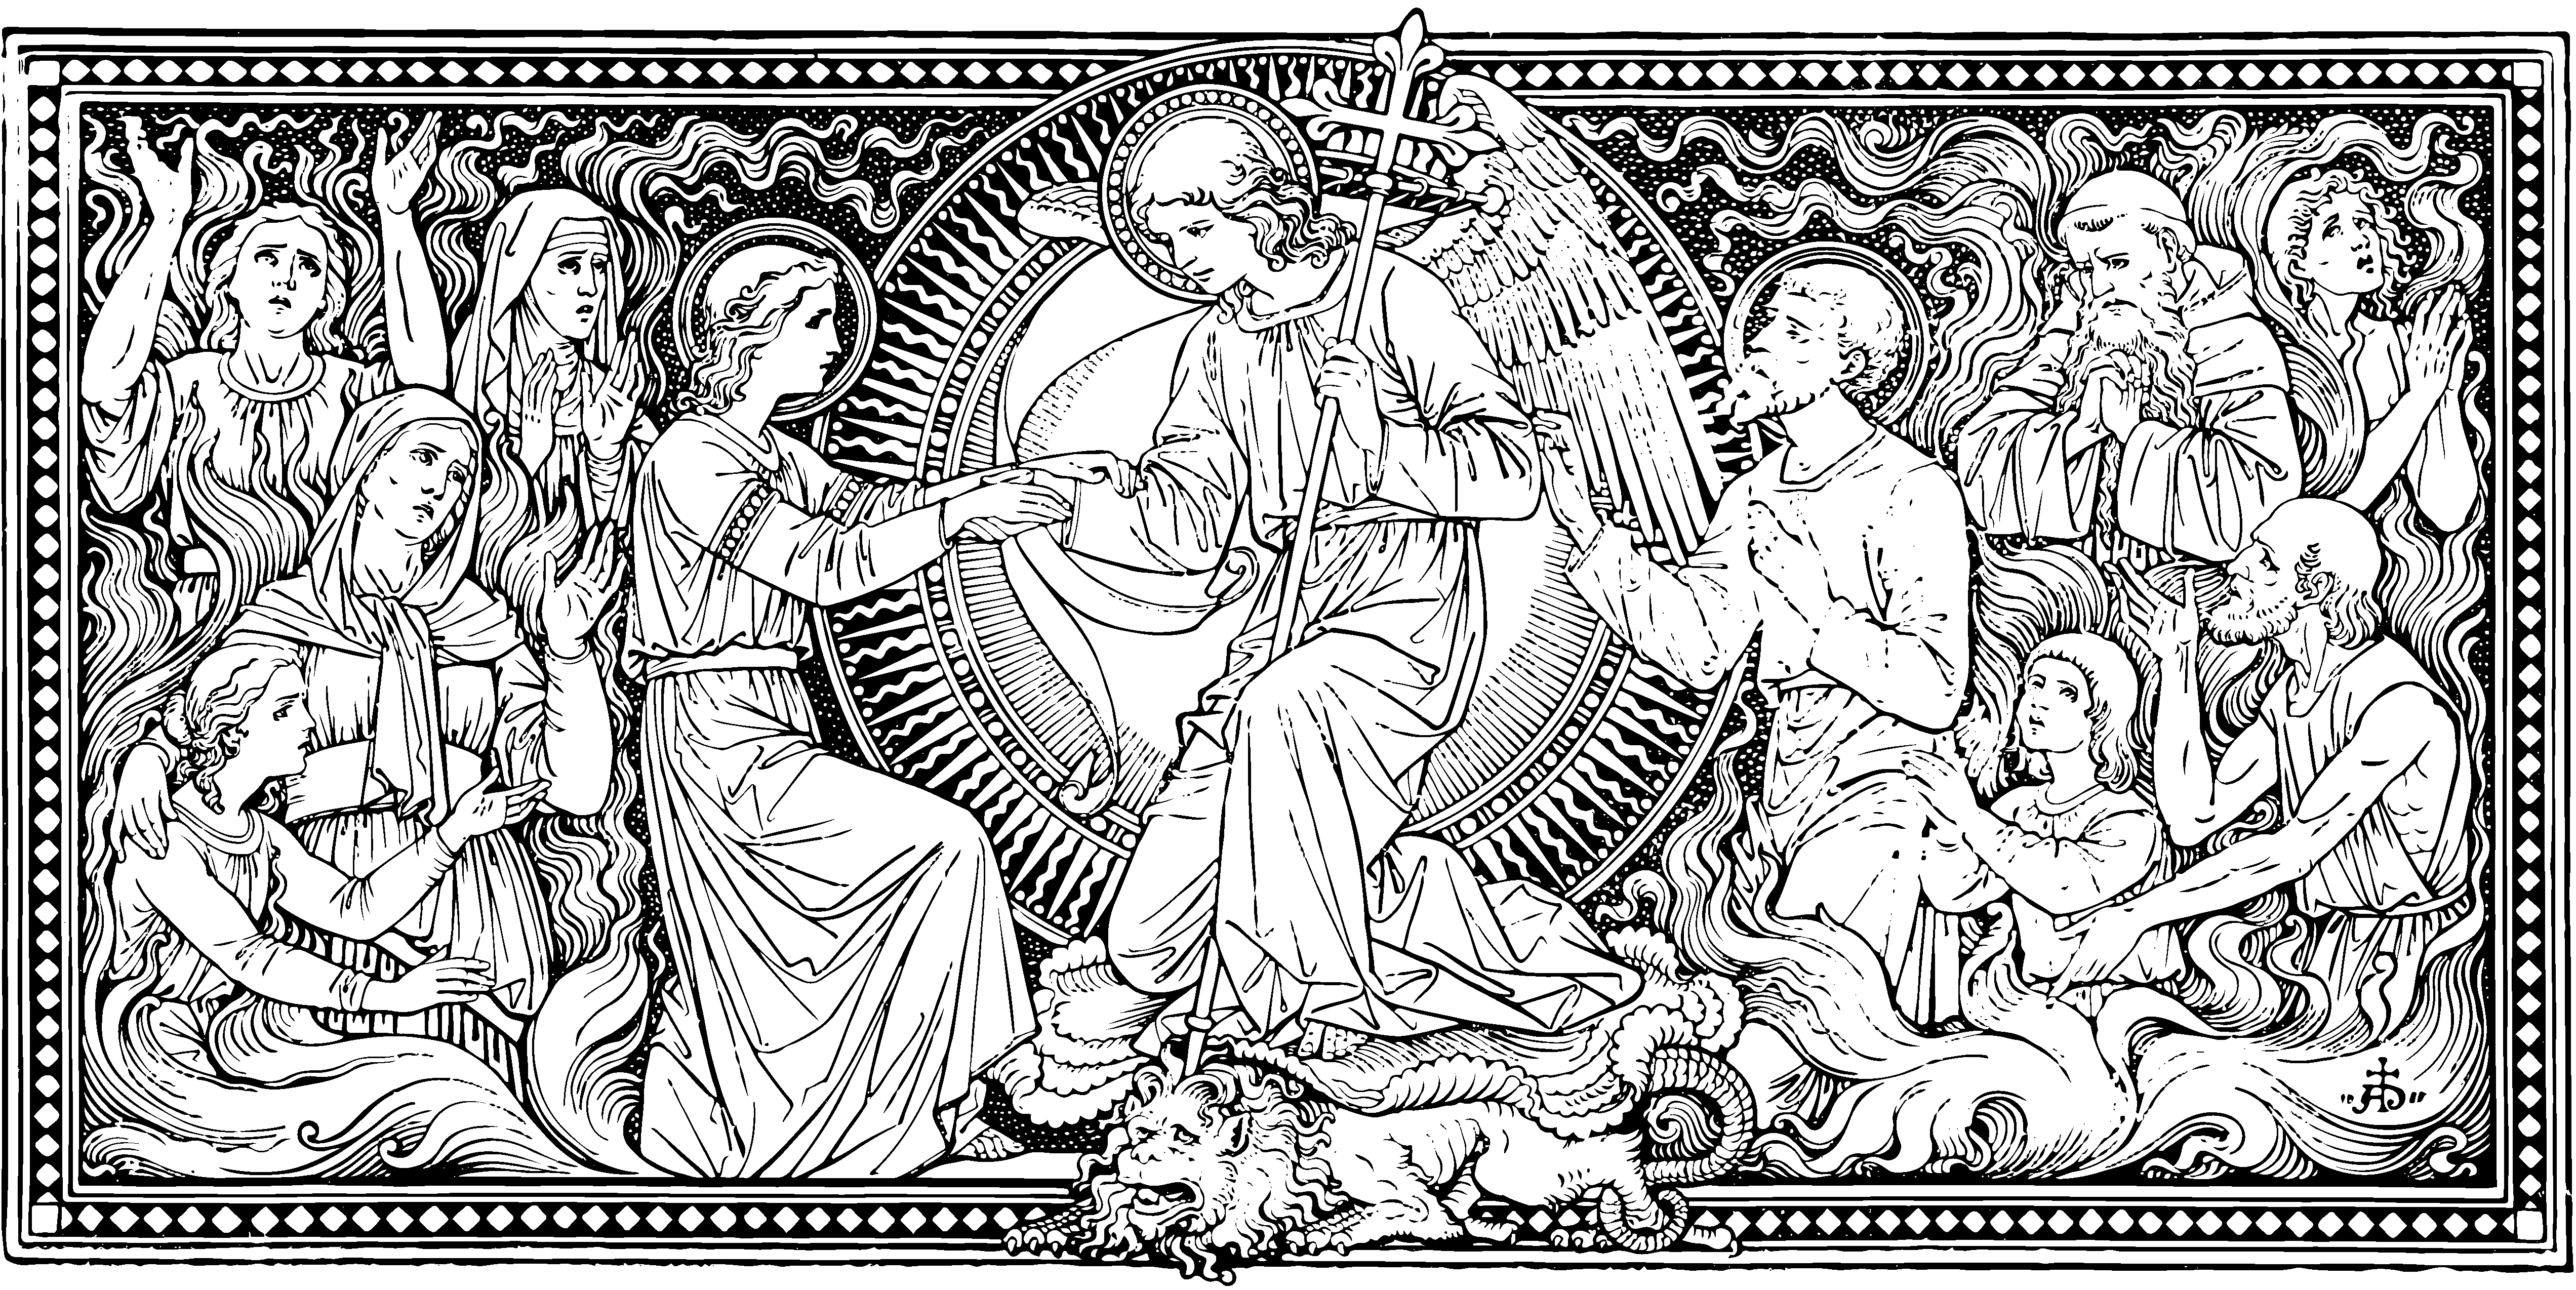
\includegraphics[width=\textwidth]{illustrations/purgatory.png}\par}
\pagebreak
\null\vspace{\baselineskip}

\rubric{Sequens Responsorium ponitur, ultimo loco, quando dicti fuerint pro Defunctis tres Nocturni.}

\vspace{5mm}

{\grechangedim{baselineskip}{62pt plus 1pt minus 5pt}{scalable}
	\gscore{ODEFN3R3b}{R}{9}{Libera me Domine de morte}
}

\vspace{\baselineskip}

\rubric{Si non sequent Laudes, dicuntur sequentes:}

\gscore[n]{ORDVb}{T}{}{Dominus vobiscum}
\rubric{vel \normaltext{Dómine, exáudi}, etc.}

\vspace{\baselineskip}

\rubric{Deinde dicitur Oratio (seu dicuntur Orationes), additis sequentibus:}

\gscore[n]{ODEFORRequiem}{T}{}{Requiem aeternam}
\gscore[n]{ODEFORRequiescant}{T}{}{Requiescant in pace}

\end{document}